\textit{You Only Look Once: Unified, Real-time Object Detection}(YOLO)\cite{yolo}是单阶段方法的开山之作。它将检测任务表述成一个统一的、端到端的回归问题,并且以只处理一次图片同时到位置和分类而得名。“One Stage”的想法就比较简单,给定一张图像,使用回归的方式输出这个目标的边框和类别。“One Stage”最核心的还是利用了分类器优秀的分类效果,首先给出一个大致的范围(最开始就是全图)进行分类,然后不断迭代这个范围直到一个精细的位置,
\begin{uscfigure}
	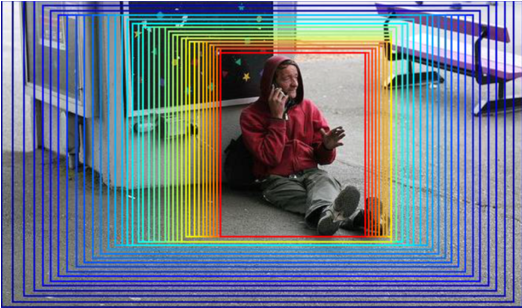
\includegraphics[width=\textwidth]{./Pictures/od_regressor.png}	
	\caption{YOLO}
	\label{yolo}
\end{uscfigure}
如图\ref{yolo}从蓝色的框框到红色的框框。这就是“One Stage”回归的思想,这样做的优点就是快,但是会有许多漏检。

\subsubsection{YOLO}
\textbf{YOLO}就是使用回归这种做法的典型算法。首先将图片Resize到固定尺寸,然后通过一套卷积神经网络,最后接上FC(全连接层)直接输出结果,这就他们整个网络的基本结构。更具体地做法,是将输入图片划分成一个SxS的网格,每个网格负责检测网格里面的物体是什么物体,并输出Bbox Info和置信度。这里的置信度指的是 该网格内含有什么物体和预测这个物体的准确度。

更具体的是如下定义:
\[
	Pr(Class_i | Object) * Pr(Object) * IOU_{pred}^{truth} = Pr(Class_i) * IOU_{pred}^{truth}
\]
这个想法其实就是一个简单的分而治之想法,将图片卷积后提取的特征图分为SxS块,然后利用优秀的分类模型对每一块进行分类,将每个网格处理完使用非极大值抑制(NMS)的算法去除重叠的框,最后得到我们的结果。
\subsubsection{SSD}
YOLO 这样做的确非常快,但是问题就在于该算法对小物体的检测效果不好。

所以SSD就在YOLO的主意上添加了Faster R-CNN的Anchor概念,并融合不同卷积层的特征做出预测。关于SSD算法的细节介绍将在第三章将详细阐述。
